\documentclass[red]{../tutorial}
\usepackage[no-math]{fontspec}
%\usepackage{xpatch}
%	\renewcommand{\ttdefault}{ul9}
%	\xpatchcmd{\ttfamily}{\selectfont}{\fontencoding{T1}\selectfont}{}{}
%	\DeclareTextCommand{\nobreakspace}{T1}{\leavevmode\nobreak\ }
\usepackage{polyglossia} % English please
	\setdefaultlanguage[variant=us]{english}
%\usepackage[charter,cal=cmcal]{mathdesign} %different font
%\usepackage{avant}
\usepackage{microtype} % Less badboxes


\usepackage[charter,cal=cmcal]{mathdesign} %different font
%\usepackage{euler}
 
\usepackage{tikz}
\usepackage{pgfplots}
\usetikzlibrary{arrows.meta}

\usepackage{blindtext}
\usepackage{calc, ifthen, xparse, xspace}
\usepackage{makeidx}
\usepackage[hidelinks, urlcolor=blue]{hyperref}   % Internal hyperlinks
\usepackage{mathtools} % replaces amsmath
\usepackage{bbm} %lower case blackboard font
\usepackage{amsthm, bm}
\usepackage{thmtools} % be able to repeat a theorem
\usepackage{thm-restate}
\usepackage{graphicx}
\usepackage{xcolor}
\usepackage{multicol}
\usepackage{fnpct} % fancy footnote spacing

 
\newcommand{\xh}{{{\mathbf e}_1}}
\newcommand{\yh}{{{\mathbf e}_2}}
\newcommand{\zh}{{{\mathbf e}_3}}
\newcommand{\R}{\mathbb{R}}
\newcommand{\Z}{\mathbb{Z}}
\newcommand{\N}{\mathbb{N}}
\newcommand{\proj}{\mathrm{proj}}
\newcommand{\Proj}{\mathrm{proj}}
\newcommand{\Perp}{\mathrm{perp}}
\newcommand{\Span}{\mathrm{span}\,}
\newcommand{\Img}{\mathrm{img}\,}
\newcommand{\Null}{\mathrm{null}\,}
\newcommand{\Range}{\mathrm{range}\,}
\newcommand{\rref}{\mathrm{rref}}
\newcommand{\Rank}{\mathrm{rank}}
\newcommand{\nnul}{\mathrm{nullity}}
\newcommand{\mat}[1]{\begin{bmatrix}#1\end{bmatrix}}
\renewcommand{\d}{\mathrm{d}}
\newcommand{\Id}{\operatorname{id}}



\theoremstyle{definition}
\newtheorem{example}{Example}[section]
\newtheorem{defn}{Definition}[section]

%\theoremstyle{theorem}
\newtheorem{thm}{Theorem}[section]

\pgfkeys{/tutorial,
	name={Tutorial 1},
	author={Bernardo Galv\~ao-Sousa},
	course={APM 348},
	date={},
	term={},
	title={Optimization}
	}

\begin{document}
	\begin{tutorial}
				\begin{objectives}
			In this tutorial you will be introduced to two fundamental tools for Mathematics and MAthematical Modelling:
				\begin{itemize}
					\item \LaTeX -- used to write documents. It is a very useful tool that makes creating scientific documents much easier and better looking.
					\item Jupyter Notebooks and Python -- Jupyter notebooks are installed in UofT servers and they include the Python programming language, so it makes programming and annotating with Python much easier
				\end{itemize}
		\end{objectives}

\vspace{-.5em}
\subsection*{Problems}
\vspace{-.5em}


\begin{enumerate}
	\item\label{q1} Work on Homework 0.

	
	
	
	
	
\end{enumerate}


















	\end{tutorial}

%	\begin{solutions}
%		\begin{enumerate}

\item First, let us define some variables:
	\begin{itemize}
		\item $x(s,w) = $ number of board games placed in shelf $s$ with size $w$ cm, for $s \in \{ 1,2,3,4\}$, and $w \in \{7,8,9\}$.
	\end{itemize}
	
We then have the following constraints:
	\begin{itemize}
		\item We have 5 games with 7cm-thick boxes: $\displaystyle \sum_{s=1}^4 x(s,7) \leq 5$
		\item We have 5 games with 7cm-thick boxes: $\displaystyle \sum_{s=1}^4 x(s,8) \leq 10$
		\item We have 5 games with 7cm-thick boxes: $\displaystyle \sum_{s=1}^4 x(s,9) \leq 4$ \\

		\item Each shelf can only contain games up to a total of 35cm thick: $\displaystyle \sum_{w=7}^9 w \cdot x(s,w) \leq 35$ for each $s \in \{1, 2,3,4\}$
		\item All variables are positive: $x(s,w)\geq 0$
	\end{itemize}
	
We want to maximize the number of games that we can place:
\begin{itemize}
	\item $\displaystyle \max \sum_{s,w} x(s,w)$
\end{itemize}
	
This is a linear programming problem, so we need to set it up in standard form:

\begin{tabular}{ll}
Objective & $\min \vec{c}^T \vec{x}$ \\
Constraints & $A \vec{x} \leq \vec{b}$
\end{tabular}

With this in mind, we construct these vectors and matrix:
\begin{itemize}
	\item $\vec{x} = \mat{x(1,7) \\ \vdots \\ x(4,7) \\\hline x(1,8) \\ \vdots \\ x(4,8) \\\hline x(1,9) \\ \vdots \\ x(4,9) }$
	\hfil and \hfil $\vec{c} = \mat{-1 \\ \vdots \\ -1}$
	\item $A = \left[ \begin{tabular}{cccc|cccc|cccc}
		1 & 1 & 1 & 1 & 0 & 0 & 0 & 0 & 0 & 0 & 0 & 0 \\
		0 & 0 & 0 & 0 & 1 & 1 & 1 & 1 & 0 & 0 & 0 & 0 \\
		0 & 0 & 0 & 0 & 0 & 0 & 0 & 0 & 1 & 1 & 1 & 1 \\ \hline
		7 & 0 & 0 & 0 & 8 & 0 & 0 & 0 & 9 & 0 & 0 & 0 \\
		0 & 7 & 0 & 0 & 0 & 8 & 0 & 0 & 0 & 9 & 0 & 0 \\
		0 & 0 & 7 & 0 & 0 & 0 & 8 & 0 & 0 & 0 & 9 & 0  \\
		0 & 0 & 0 & 7 & 0 & 0 & 0 & 8 & 0 & 0 & 0 & 9 
		\end{tabular} \right]$	
	\hfil and \hfil $\vec{b} = \mat{5\\10\\4\\\hline35\\35\\35\\35}$
\end{itemize}

We can then use \texttt{python} and the function \texttt{optimize.linprog} to find the minimum.

We get t he following solution:

\begin{minipage}{.3\textwidth}
\begin{itemize}
	\item $\vec{x} = \mat{ 0 \\ 0 \\ 5 \\ 0 \\\hline 4.375 \\ 1.25 \\ 0 \\ 4.375 \\\hline 0 \\ 2.77777778 \\ 0 \\ 0 }$
\end{itemize}	
\end{minipage}
\hfill \begin{minipage}{.6\textwidth}
This is a problem because we can't divide game boxes, so we need to search for integer solutions only, which require a whole different set of techniques (like the simplex method). 
Fortunately, the function \texttt{optimize.linprog} can already solve this problem if we add the option \texttt{integrality=np.ones(4*3)} to declare which of the variables should have integer values.	
\end{minipage}

We then obtain the solution:

\begin{minipage}{.2\textwidth}
	\begin{itemize}
		\item $\vec{x} = \mat{5 \\ 0 \\ 0 \\ 0  \\\hline 0 \\ 3 \\ 4 \\ 1 \\\hline 0 \\ 1 \\ 0 \\ 3}$
	\end{itemize}
\end{minipage}
\hfil 
\begin{minipage}{.5\textwidth}
	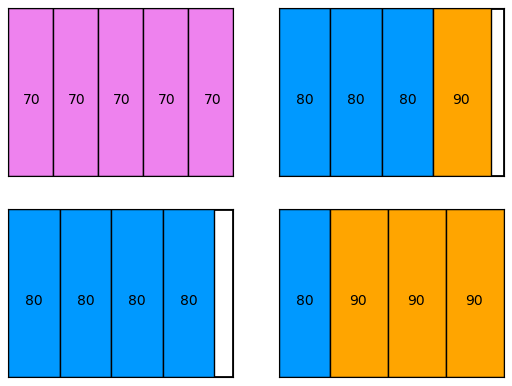
\includegraphics[width=\textwidth]{boardgame.png}
\end{minipage}


\paragraph{Extra analysis.} The function \texttt{optimize.linprog} keeps track of some extra information:

The residuals from each constraint in the variable \texttt{sol.ineqlin.residual}:
	\begin{itemize}
		\item Games residual with width 7 cm = 0
		\item Games residual with width 8 cm = 2 \hfill (2 games with 8cm-thick box not placed)
		\item Games residual with width 9 cm = 0 \\
		
		\item Shelf residual  top - left  is  0.0 cm
		\item Shelf residual  top - right  is  2.0 cm \hfill (this shelf still has 2cm of space unused)
		\item Shelf residual  bottom - left  is  3.0 cm \hfill (this shelf still has 3cm of space unused)
		\item Shelf residual  bottom - right  is  0.0 cm
	\end{itemize}

\begin{enumerate}	
\item[(c)] Just as we did with the farming problem in lectures, we can look at the ``shadow costs''. These are stored in the variable \texttt{sol.ineqlin.marginals}:
	\begin{itemize}
		\item Shadow-games with width 7 cm = 0.0
		\item Shadow-games with width 8 cm = 0.0
		\item Shadow-games with width 9 cm = 0.0 \\
		
		\item Shadow-shelf  top - left  is  0.0 games/cm
		\item Shadow-shelf  top - right  is  0.0 games/cm
		\item Shadow-shelf  bottom - left  is  0.0 games/cm
		\item Shadow-shelf  bottom - right  is  0.0 games/cm
	\end{itemize}

These are all 0 because we are requiring the solution to have integer solutions, so a small change in any constraint will not affect the solution at all. \\

However, if we change one shelf be 1cm (different from a small change), then we get the following results:


\hspace{-1em}\begin{tabular}{|c|c|c|}
\cline{1-1}\cline{3-3}
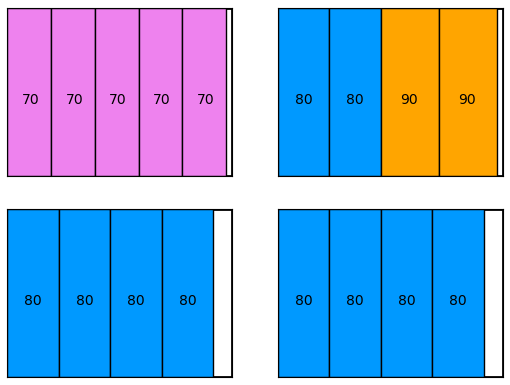
\includegraphics[width=.42\textwidth]{boardgame36a.png}
	& \qquad & 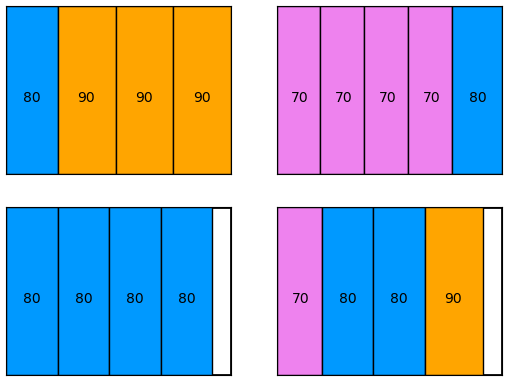
\includegraphics[width=.42\textwidth]{boardgame36b.png} \\%[-5pt]
1$^{\rm st}$ shelf is 36cm wide
	& & 2$^{\rm nd}$ shelf is 36cm wide \\ \cline{1-1}\cline{3-3}
\end{tabular}

\hfill 

Observe that although the two problems should be equivalent, the solutions found are different:
\begin{itemize}
	\item Both still put all 7cm-wide games
	\item The first one, leaves \textbf{two} 9cm-wide games unplaced
	\item The second one, only leaves \textbf{one} 8-cm game unplaced
\end{itemize}

The difference in these two solutions is due to either the programming of the algorithms or the algorithms themselves.

The second solution is clearly the better one, so we can conclude that adding 1cm to one of the shelves does change the problem significantly and allows us to place one more game in the bookshelf.
\end{enumerate}



\newpage

		
\item This is a more open ended problem, so we must first define our problem clearly.


\paragraph{Define the problem. } For the sake of this solution, we will focus on the following problem:
\begin{itemize}
	\item Given a resting position for the elevators, and all the possible cases of people calling for the elevator, we will minimize the total time the person calling the elevator needs to wait for the nearest elevator to arrive.
\end{itemize}

\paragraph{Assumptions. } We assume that each person will make two trips:
\begin{itemize}
	\item One from their apartment to the ground floor
	\item One from the ground floor to their apartment
	\item The elevator's speed is 1 floor/sec
	\item The elevator doors take 1 second to open/close
\end{itemize}
 
 We are disregarding several facts:
 \begin{itemize}
 	\item The elevator capacity	
 	\item The fact that at some times of the day (like morning), most people will take the elevator to go to the ground floor
 	\item $\cdots$
 \end{itemize}

\paragraph{Build the model.} We have the following:
\begin{itemize}
	\item There are $30\times10\times2 = 600$ people living in the building
	\item The total number of trips are 1200
	\item 600 trips from the ground floor
	\item 20 trips from each floor of the building
	\item On each trip, the person has to wait only for hte doors to open once the elevator arrives to their floor
\end{itemize}

Define:
\begin{itemize}
	\item $x_i = $ the resting position of elevator $i$
	\item for simplicity, assume that $0 \leq x_1 \leq x_2 \leq x_3$
\end{itemize}

Then we want to solve:
\[
\min_{x_1, x_2, x_3} \left[ 600 \cdot (1+x_1) + \sum_{n=1}^{30} 20 \cdot \left( 1 + \min\big\{ |n-x_1|, |n-x_2|, |n-x_3|\big\} \right) \right]
\]

\paragraph{Assess. } This is an \textbf{unconstrained minimization} problem, but it is complicated by the fact that the function includes a minimum between three values and with absolute values. It can still be solved, but it would involve dividing it into several cases to calculate the partial derivatives of the min function.  % as in the following different way to rewrite it:
%
%We can also rewrite it as follows:
%\begin{multline*}
%\min_{x_1, x_2, x_3} \Bigg[ 
%	600 \cdot x_1 
%	+ 20 \cdot \sum_{n=1}^{x_1} 20 (x_1-n)
%	+ 20 \cdot \sum_{n=x_1+1}^{\frac{x_1+x_2}{2}} (n-x_1)
%	+ 20 \cdot \sum_{n=\frac{x_1+x_2}{2}}^{x_2} (x_2-n) \\
%	+ 20 \cdot \sum_{n=x_2+1}^{\frac{x_2+x_3}{2}} (n-x_2)
%	+ 20 \cdot \sum_{n=\frac{x_2+x_3}{2}}^{x_3} (x_3-n)
%	 + 20 \cdot \sum_{n=x_3+1}^{30} (n-x_3)
%	\Bigg]
%\end{multline*}

Instead, we use \texttt{optimize.fmin}\footnote{We also need to penalize the function when it ``wants'' to have negative values of $x_i$.} to get 
\begin{itemize}
	\item $x_1 = 4.371016527455962e-08$
	\item $x_2 = 12.106232494580468$
	\item $x_3 = 24.000002224317633$
	\item Total time $= 2940.000066 $ seconds $= 49$ minutes
\end{itemize}

Because it would be strange to keep the elevators between floors (although it's possible), we can check the nearby values for the optimal solution:

%\begin{minipage}{.45\textwidth}
\begin{itemize}
	\item $x_1 = 0$
	\item $x_2 = 12$
	\item $x_3 = 24$
	\item Total time $= 2940$ sec $= 49$ min
\end{itemize}	
%\end{minipage}
%\begin{minipage}{.45\textwidth}
%\begin{itemize}
%	\item $x_1 = 0$
%	\item $x_2 = 11$
%	\item $x_3 = 24$
%	\item Total time $= 1740$ sec $= 29$ min
%\end{itemize}
%\end{minipage}

Here are two graphs with the time function we are minimizing and the elevators as they are placed in the building.

\hspace{-3em}\begin{tabular}{ccc}
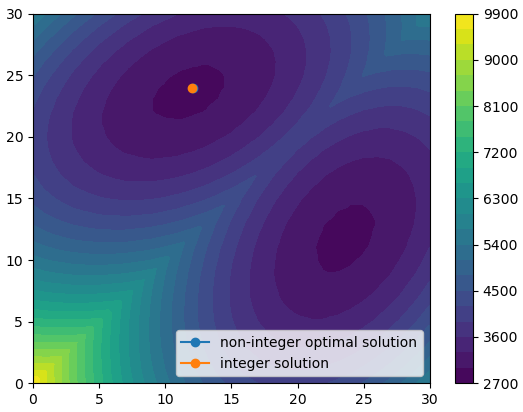
\includegraphics[height=200pt]{elevators-time.png}
	& & 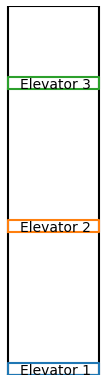
\includegraphics[height=200pt]{elevators-building.png} \\[-5pt]
The time function with $x_1=0$
	& & The building with the elevators
\end{tabular}

\hfill 


\begin{enumerate}
\item[(c)] We check the sensitivity of this problem with respect to some of the parameters.

\begin{itemize}
	\item Sensitivity with respect to number of people living in each floor:
		\[S(T^\star, {\rm Ppf}) \approx 1\]
	\item Sensitivity with respect to time it takes the elevators to open/close the doors:
		\[S(T^\star, E_s) \approx 0.41\]
\end{itemize}
\end{enumerate}




		
			
\end{enumerate}
	

%	
%	\end{solutions}
%	\begin{instructions}
%		\subsection*{Learning Objectives}
	Students need to be able to\ldots
	\begin{itemize}
		\item Model optimization problems. \\[-20pt]
		\item Recognize what type of optimization problem they need.\\[-20pt]
		\item Use \texttt{Jupyter Notebook} to approximate the solution.\\[-20pt]
		\item Create a visualization of the problem and the solution.
	\end{itemize}

\subsection*{Context}
	
In lecture we have been studying different types of optimization problems:
\begin{itemize}
	\item Unconstrained optimization
	\item Constrained optimization (Lagrange multipliers)
	\item Linear programming
	\item Calculus of Variations (Euler-Lagrange equations)
\end{itemize}

We have also introduced some extra ways to study optimization problems:
\begin{itemize}
	\item Sensitivity of the objective function with respect to a parameter
	\item ``Shadow-cost'' and the meaning of Lagrange multiplier values
\end{itemize}

In this class, we want to study new problems and make use of these extra ideas to study how the problem and its solution changes when we change parameters. \\


In this tutorial, we will do the following:
\begin{itemize}
	\item Define what we want to optimize
	\item Model and approximate the solution using \texttt{python} tools
	\item Visualize the solutions
	\item Assess the solutions
\end{itemize}


\paragraph{Important.} Don't rush problem 1 to be able to get to problem 2. Even if the students only have time to think about defining the problem and setting assumptions for problem 2, that's ok!


\subsection*{Resources for TAs}

Some \texttt{Jupyter Notebook} scripts:

\begin{itemize}
	\item Boardgame problem \ref{q1}: \href{https://utoronto.syzygy.ca/jupyter/user-redirect/git-pull?repo=https://github.com/bigfatbernie/IBLMathModeling&subPath=tutorials/tutorial2/boardgame-linearprog.ipynb}{\tt boardgame-linearprog.ipynb}
	\item Elevator problem \ref{q2}: \href{https://utoronto.syzygy.ca/jupyter/user-redirect/git-pull?repo=https://github.com/bigfatbernie/IBLMathModeling&subPath=tutorials/tutorial2/elevators.ipynb}{\tt elevators.ipynb}
\end{itemize}


\subsection*{Before Tutorial}

Send an announcement to students letting them know that they will need to bring a laptop and will be using Jupyter Notebooks \url{https://utoronto.syzygy.ca}.


\subsection*{What to Do}
	
Introduce the learning objectives for the day's tutorial. \\

Have students get into small groups and start on \#1 -- each group needs to have at least 1 laptop. 

The first problem should be very self explanatory. Students should be able to do it without hints. \\

On part (b), students should be able to report on how many games go into each shelf instead of just showing with the solution vector is.\\

On part (c), observe that depending on where we put the defective shelf, the computer will give us different results -- some clearly not optimal. 

Students should be aware that even though some problems are ``symmetric'', the methods we use to approximate might not be, so they should plan to check solutions that in theory should be the same.


\hfill 

The second question is open ended and students will probably struggle to define a problem to optimize.

Some key ways to help students:
\begin{itemize}
	\item Students should think of a problem related to the elevator function that they \textbf{CAN} optimize -- this means they'll have to make simplifying assumptions.
	\item Hint \#1: Assume a ``static'' elevator problem, where the elevators are in a position (to be optimized) waiting to be called
	\item Hint \#2: What kinds of trips do people in an apartment building make? -- look towards simplifying assumptions
\end{itemize}

Be open to students having different models and different objectives, as long as they are actionable.

	


%\subsection*{Notes}
%
%	\begin{enumerate}
%		\item Note
%	\end{enumerate}
	
	

	
	

%	\end{instructions}

\end{document}
